\chapter{Signaleigenschaften}

In diesem Kapitel werden Eigenschafen von kausalen und analytischen Signalen abgehandelt.\\

\paragraph{Stabilität} von einem Signal $x(t)$ ist gegeben wenn
\begin{equation}
\int_{-\infty}^\infty |x(t)|^2\,dt < \infty.
\end{equation}

\section{Kausalität eines Signals}
Kausalität eines Signals ist erfüllt wenn:
\[
\begin{split}
f(t) = 0 ,&\:t \leq 0\\
\int_0^\infty f(t)^2\,dt > 0,&\:t > 0
\end{split}
\]
\textit{Kausal} bedeutet hier wenn es sich um eine physikalisch realisierbares System handelt. Also kein Wirkung vor der Ursache stattfindet.

\subsection{Physikalisch Realisierbares System}
Ein physikalisch realisierbares System ist gegeben wenn:
\begin{equation}
\begin{split}
y(t) = f(t) * x(t) & = \int_{-\infty}^\infty f(t')\, x(t-t') dt'\\
& =\int_0^\infty f(t')\, x(t-t') dt'
\end{split}
\end{equation}
Wobei $y(t)$ der Output des Systems $f(t)$ mit dem Input $x(t)$ ist. Weiter ist $t' \geq 0$, d.h. es wird nur auf aktielle und vergangene Werte des Inputs zugegriffen.

%\section{Eigenschaften eines Kausalen Systems}
%Welche Eigenschaften hat das Spektrum eines kausalen Systems?

\section{Hilberttransformation}
Die Hilberttransformation ist eine Phasenverschiebung des Signals um 90$^\circ$. Die passiert zum Beispiel wenn eine Welle durch eine Kaustik, ein Brennpunkt mehrer Wellenpfade, läuft, oder bei der Reflektion an Schichtgrenzen mit Negativer Impendanz.\\
Definition der Hilberttransformation.
\begin{equation}
H\{x(t)\} = \frac{1}{\pi} \int_{-\infty}^\infty \frac{x(t')}{t'-t}\,dt' = x_H(t)
\end{equation}
Problem wenn $t'=t$, dann tritt Singularität auf.\\
Die Lösung ist das Integral im Sinne des Couchy'schen Hauptwerdes zu bilden:
\begin{equation}
H\{x(t)\} = \frac{1}{\pi}\,\lim_{\epsilon \rightarrow 0} \left(\int_{-\infty}^{t-\epsilon} \frac{x(t')}{t'-t}\,dt' + \int_{t+\epsilon}^{\infty} \frac{x(t')}{t'-t}\,dt' \right)
\end{equation}
Wobei für $\epsilon > 0$ gilt.\\\\
Die Rücktransformation der Hilbertransformation ist wie folgt:
\begin{equation}
H^{-1}\{x_H(t)\} = x(t) = -\frac{1}{\pi} \int_{-\infty}^\infty \frac{x_H(t')}{t'-t}\,dt'
\end{equation}

\paragraph{Beispiel der Hilbertransformation} für harmonische Sinusfunktion
\[
\begin{split}
H\{-\sin (\omega_0t)\} = & \cos (\omega_0 t)\\
H\{\cos (\omega_0t)\} = & \sin (\omega_0 t)
\end{split}
\]

\subsection*{Hilberttransformation durch Faltung}
Die Hilberttransformation kann durch Faltung dargestellt werden:
\[
H\{x(t)\} = -\frac{1}{\pi t} * x(t)
\]

\subsection*{Hilberttransformation im Frequenzbereich}
Die Hiblerttransformation im Frequenzbereich,
\[
F\{H\{x(t)\}\} = i\,\mbox{sign}\,\omega\,X(\omega)
\]
Dabei ist $i\,\mbox{sign}\,\omega = 
\begin{cases}
-i & \omega < 0\\
i & \omega \geq 0
\end{cases}$

\subsection*{Berechnung der Hilberttransformation}
Die praktische Berechnung der Hilberttransformation über den analytische Zerlegung des Signals in den Frequenzbereich.
\[
\begin{split}
F\{x(t)\} = & X(\omega)\\
i\,\mbox{sign}\,\omega\,X(\omega) = &F\{H\{x(t)\}\}\\
\end{split}
\]
So ist
\[
F^{-1}\{i\,\mbox{sign}\,\omega\,X(\omega)\} = x_H(t)
\]
die Hilberttransformation des Signals $x(t)$

\section{Analytische und Reelle Signale}
Das Signal ist definiert als
\[
y(t) = x(t) - i\,H\{x(t)\}.
\]
Durch Fourier Transformation erhalten wir
\[
\begin{split}
Y(\omega) & = X(\omega) - i \, \mbox{sign}\,\omega \, X(\omega)\\
& = X(\omega) + \mbox{sign}\,\omega \, X(\omega)\\
& =
\begin{cases}
2 X(\omega) & \omega \geq 0\\
0 & \omega < 0
\end{cases}
\end{split}
\]
Das bedeutet, dass das Spektrum eines analytischen Signals kausal ist - Sowie das Spektrum eines kausalen Signals analytisch ist!

\subsection{Berechnung eines analytischen Signals}
Das analytische Signal kann im Frequenzbereich berechnet werden.
\[
\begin{split}
F\{x(t)\} = & X(\omega)\\
\rightarrow Y(\omega) =
\begin{cases}
2 X(\omega) & \omega \geq 0\\
0 & \omega < 0
\end{cases}
\end{split}
\]

\subsection{Berechnung der Envelope}
\label{sec:signalyse_envelope}
Die Envelope des Signals ist die \textit{Einhüllende} der Signalreihe. Die Envelope ist definiert als
\begin{equation}
E(t) = |y(t)|,
\end{equation} 
der Betrag des \textit{analytischen} Signals.
\begin{figure}[h!]
\centering
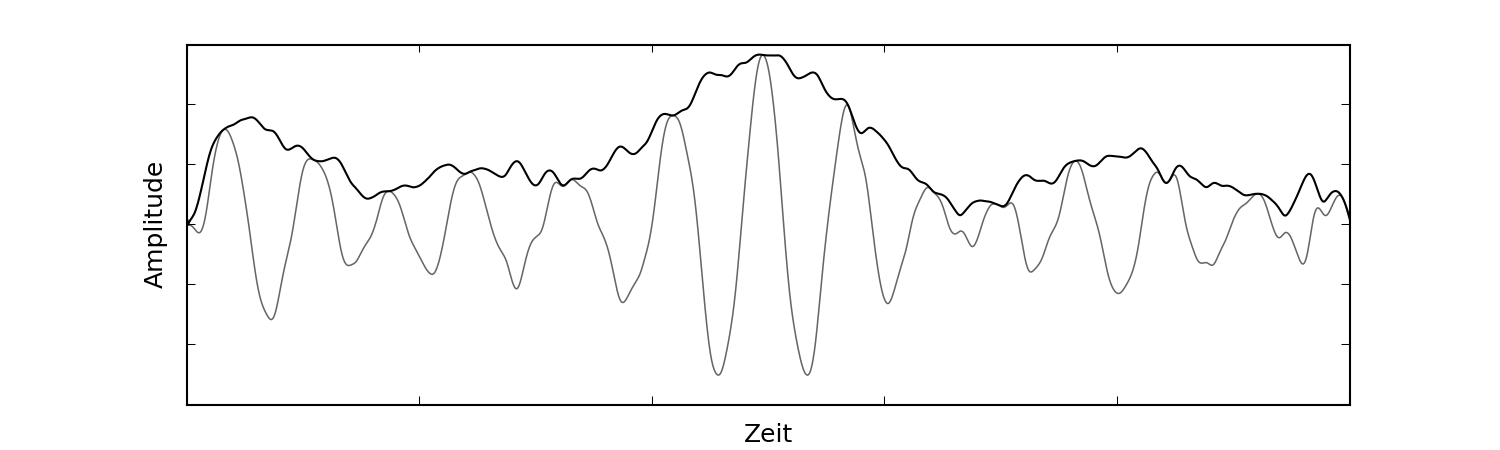
\includegraphics[width=.9\tw]{fig/08-Signalanalyse/envelope.png}
\caption{Die Einhüllende (Envelope) des Signals.}
\end{figure}


\subsection{Beispiele}
Sei das Signal definiert als:
\[
\begin{split}
x(t) & = a\, \cos (\omega_0 t)\\
y(t) & = a\, \cos(\omega_0 t) - i\, a\, \sin (\omega_0 t)
\end{split}.
\]
Dabei ist $x(t)$ das reelle und $y(t)$ das analytische Signal.

\paragraph{Die Envelope} des Signals ist
\[
E(t) = |y(t)| = a.
\]

\paragraph{Die Phase} des Signals ist
\[
\phi(t) = \omega_0 t.
\]

\paragraph{Die Momentane Frequenz} des Signals bei $t$ ist
\[
\omega(t) = \frac{d \phi(t)}{d t}.
\]
Was in diesem analytischen System $\omega(t) = \omega_0$ ist.\\\\
Die Änderung der Phase kann die Ankunft eines Signals durch Spikes in $\frac{d \phi(t)}{d t}$ anzeigen.

\paragraph{Die Momentane Phase} des Signals bei $t$ ist
\[
\phi(t) = \arctan\left( \frac{Im\{y(t)\}}{Re\{y(t)\}} \right)
\]
\subsection{Konstruktion eines kausalen Signals}
Konstruktion eines kausalen, nullphasigen Signals für ein gegebenes Amplitudenspektrum.
\[
\begin{split}
F(\omega) & = |F(\omega)|\, e^{-\phi(\omega)}\\
G(\omega) & = \ln(F(\omega)) = \ln(|F(\omega)| + i\,\phi(\omega)
\end{split}
\]
Durch $\ln$ haben wir die Form des analytischen Signals.\\\\
Die Phase kann aus dem Amplitudenspektrum berechnet werden.
\[
\phi(\omega) = -H\{\ln(|F(\omega)|\}
\]